% Options for packages loaded elsewhere
\PassOptionsToPackage{unicode}{hyperref}
\PassOptionsToPackage{hyphens}{url}
%
\documentclass[
]{book}
\usepackage{amsmath,amssymb}
\usepackage{lmodern}
\usepackage{iftex}
\ifPDFTeX
  \usepackage[T1]{fontenc}
  \usepackage[utf8]{inputenc}
  \usepackage{textcomp} % provide euro and other symbols
\else % if luatex or xetex
  \usepackage{unicode-math}
  \defaultfontfeatures{Scale=MatchLowercase}
  \defaultfontfeatures[\rmfamily]{Ligatures=TeX,Scale=1}
\fi
% Use upquote if available, for straight quotes in verbatim environments
\IfFileExists{upquote.sty}{\usepackage{upquote}}{}
\IfFileExists{microtype.sty}{% use microtype if available
  \usepackage[]{microtype}
  \UseMicrotypeSet[protrusion]{basicmath} % disable protrusion for tt fonts
}{}
\makeatletter
\@ifundefined{KOMAClassName}{% if non-KOMA class
  \IfFileExists{parskip.sty}{%
    \usepackage{parskip}
  }{% else
    \setlength{\parindent}{0pt}
    \setlength{\parskip}{6pt plus 2pt minus 1pt}}
}{% if KOMA class
  \KOMAoptions{parskip=half}}
\makeatother
\usepackage{xcolor}
\usepackage{color}
\usepackage{fancyvrb}
\newcommand{\VerbBar}{|}
\newcommand{\VERB}{\Verb[commandchars=\\\{\}]}
\DefineVerbatimEnvironment{Highlighting}{Verbatim}{commandchars=\\\{\}}
% Add ',fontsize=\small' for more characters per line
\usepackage{framed}
\definecolor{shadecolor}{RGB}{248,248,248}
\newenvironment{Shaded}{\begin{snugshade}}{\end{snugshade}}
\newcommand{\AlertTok}[1]{\textcolor[rgb]{0.94,0.16,0.16}{#1}}
\newcommand{\AnnotationTok}[1]{\textcolor[rgb]{0.56,0.35,0.01}{\textbf{\textit{#1}}}}
\newcommand{\AttributeTok}[1]{\textcolor[rgb]{0.77,0.63,0.00}{#1}}
\newcommand{\BaseNTok}[1]{\textcolor[rgb]{0.00,0.00,0.81}{#1}}
\newcommand{\BuiltInTok}[1]{#1}
\newcommand{\CharTok}[1]{\textcolor[rgb]{0.31,0.60,0.02}{#1}}
\newcommand{\CommentTok}[1]{\textcolor[rgb]{0.56,0.35,0.01}{\textit{#1}}}
\newcommand{\CommentVarTok}[1]{\textcolor[rgb]{0.56,0.35,0.01}{\textbf{\textit{#1}}}}
\newcommand{\ConstantTok}[1]{\textcolor[rgb]{0.00,0.00,0.00}{#1}}
\newcommand{\ControlFlowTok}[1]{\textcolor[rgb]{0.13,0.29,0.53}{\textbf{#1}}}
\newcommand{\DataTypeTok}[1]{\textcolor[rgb]{0.13,0.29,0.53}{#1}}
\newcommand{\DecValTok}[1]{\textcolor[rgb]{0.00,0.00,0.81}{#1}}
\newcommand{\DocumentationTok}[1]{\textcolor[rgb]{0.56,0.35,0.01}{\textbf{\textit{#1}}}}
\newcommand{\ErrorTok}[1]{\textcolor[rgb]{0.64,0.00,0.00}{\textbf{#1}}}
\newcommand{\ExtensionTok}[1]{#1}
\newcommand{\FloatTok}[1]{\textcolor[rgb]{0.00,0.00,0.81}{#1}}
\newcommand{\FunctionTok}[1]{\textcolor[rgb]{0.00,0.00,0.00}{#1}}
\newcommand{\ImportTok}[1]{#1}
\newcommand{\InformationTok}[1]{\textcolor[rgb]{0.56,0.35,0.01}{\textbf{\textit{#1}}}}
\newcommand{\KeywordTok}[1]{\textcolor[rgb]{0.13,0.29,0.53}{\textbf{#1}}}
\newcommand{\NormalTok}[1]{#1}
\newcommand{\OperatorTok}[1]{\textcolor[rgb]{0.81,0.36,0.00}{\textbf{#1}}}
\newcommand{\OtherTok}[1]{\textcolor[rgb]{0.56,0.35,0.01}{#1}}
\newcommand{\PreprocessorTok}[1]{\textcolor[rgb]{0.56,0.35,0.01}{\textit{#1}}}
\newcommand{\RegionMarkerTok}[1]{#1}
\newcommand{\SpecialCharTok}[1]{\textcolor[rgb]{0.00,0.00,0.00}{#1}}
\newcommand{\SpecialStringTok}[1]{\textcolor[rgb]{0.31,0.60,0.02}{#1}}
\newcommand{\StringTok}[1]{\textcolor[rgb]{0.31,0.60,0.02}{#1}}
\newcommand{\VariableTok}[1]{\textcolor[rgb]{0.00,0.00,0.00}{#1}}
\newcommand{\VerbatimStringTok}[1]{\textcolor[rgb]{0.31,0.60,0.02}{#1}}
\newcommand{\WarningTok}[1]{\textcolor[rgb]{0.56,0.35,0.01}{\textbf{\textit{#1}}}}
\usepackage{longtable,booktabs,array}
\usepackage{calc} % for calculating minipage widths
% Correct order of tables after \paragraph or \subparagraph
\usepackage{etoolbox}
\makeatletter
\patchcmd\longtable{\par}{\if@noskipsec\mbox{}\fi\par}{}{}
\makeatother
% Allow footnotes in longtable head/foot
\IfFileExists{footnotehyper.sty}{\usepackage{footnotehyper}}{\usepackage{footnote}}
\makesavenoteenv{longtable}
\usepackage{graphicx}
\makeatletter
\def\maxwidth{\ifdim\Gin@nat@width>\linewidth\linewidth\else\Gin@nat@width\fi}
\def\maxheight{\ifdim\Gin@nat@height>\textheight\textheight\else\Gin@nat@height\fi}
\makeatother
% Scale images if necessary, so that they will not overflow the page
% margins by default, and it is still possible to overwrite the defaults
% using explicit options in \includegraphics[width, height, ...]{}
\setkeys{Gin}{width=\maxwidth,height=\maxheight,keepaspectratio}
% Set default figure placement to htbp
\makeatletter
\def\fps@figure{htbp}
\makeatother
\setlength{\emergencystretch}{3em} % prevent overfull lines
\providecommand{\tightlist}{%
  \setlength{\itemsep}{0pt}\setlength{\parskip}{0pt}}
\setcounter{secnumdepth}{5}
\usepackage{booktabs}
\ifLuaTeX
  \usepackage{selnolig}  % disable illegal ligatures
\fi
\usepackage[]{natbib}
\bibliographystyle{apalike}
\IfFileExists{bookmark.sty}{\usepackage{bookmark}}{\usepackage{hyperref}}
\IfFileExists{xurl.sty}{\usepackage{xurl}}{} % add URL line breaks if available
\urlstyle{same} % disable monospaced font for URLs
\hypersetup{
  pdftitle={Quantitative Methods in Educational Research Using R},
  pdfauthor={Subash Parajuli},
  hidelinks,
  pdfcreator={LaTeX via pandoc}}

\title{Quantitative Methods in Educational Research Using R}
\author{Subash Parajuli}
\date{2023-02-08}

\begin{document}
\maketitle

{
\setcounter{tocdepth}{1}
\tableofcontents
}
\hypertarget{syllabus}{%
\chapter{Syllabus}\label{syllabus}}

EIPT 5023 -- Analysis of Quantitative Data I, Fall 2022

\textbf{Course Description:} This course covers descriptive and basic inferential statistics, including graphs, frequency distributions, central tendency, dispersion, probability, hypothesis testing, tests of mean differences, correlation and simple regression, and chi-square tests. Computer applications are included.

\textbf{Course Overview:} This course is designed to provide students with an opportunity to develop their knowledge and understanding of various statistical concepts and procedures. In particular, it is hoped that students will leave the course with (a) a recognition of how statistics fits within the broader (quantitative) research process, (b) an understanding of the assumptions associated with different statistical procedures and how those assumptions should guide analytic choices, and (c) an understanding of how to utilize tools (such as SPSS) in order to analyze quantitative data.

\hypertarget{general-objectives}{%
\chapter{\texorpdfstring{\textbf{General Objectives:}}{General Objectives:}}\label{general-objectives}}

To be able to correctly identify variables falling at different scales of measurement.

To be able to correctly identify appropriate techniques for analyzing data when presented with variables with different measurement characteristics.

To be able to understand the assumptions associated with different statistical tests.

To be able to set up and manage databases containing variables.

To be able to carry out statistical analyses of data using SPSS.

To be able to correctly interpret the results of statistical analyses.

To be able to distinguish between null and alternative (research) hypotheses.

To be able to distinguish between a directional and non-directional hypothesis.

To understand the concepts of "statistical significance" and "effect size".

To understand the effects of sampling (e.g., size, strategies) on inferences concerning population estimates.

\hypertarget{why-read-statistics}{%
\chapter{Why read Statistics?}\label{why-read-statistics}}

As a field, statistics is concerned with the analysis of numerical data (which has either

been collected by a researcher or organization). Data analysis is generally carried out

for the purposes of defining problems and/or making decisions to address problems.

Examples where statistics could be used in decision-making:

During election season, polling organizations may ask people in the public who

they are likely to vote for (e.g., Candidate A versus Candidate B). They may

compute various statistics to come up with a prediction of who is most likely to

win an election. This information may be presented in newspapers, on the

internet, or in other media.

Similarly, the candidates themselves (or people on their behalf) may carry out polls

to determine what issues are most important to the public and shape their

message accordingly. This often entails analysis of numerical data (e.g., from

surveys).

A marketer may collect data on peoples' buying habits at a store (e.g., people who

purchase product A also tend to purchase product B) in order to market products

to potential customers.

A medical researcher might carry out statistical analysis of data in order to

determine which drug (either drug A or drug B) is more beneficial in managing pain

associated with cancer.

An educational researcher may use statistical analysis of data in order to test

models aimed at predicting academic achievement in students. The

researcher may obtain measures of Mastery goal orientation, Cognitive

Engagement, and Self-efficacy and use these as predictors of performance on

an achievement test.

A criminal justice researcher might be interested in determining what kinds

of individual difference factors (e.g., empathy, neuroticism, openness) are

associated with an increased likelihood a person will engage in criminal

activity. The researcher might obtain data from a number of individuals and

test relationships among certain variables using statistical analysis. This might

be useful for developing interventions to decrease the likelihood of a person

engaging in criminal activity.

Legislators (or people on their behalf) might carry out statistical analyses in

order to better understand where and how to allocate funds for education,

the military, etc.

As you can see, statistics is applied in many different fields to address both theoretical

and practical questions. Based on interpretation of data, stakeholders can use this

information for planning purposes, the development of interventions, or gaining a

better understanding of certain phenomena.

Importantly, even if you do not carry out statistical analyses of data yourself, you still

are being influenced by others who use statistics. When you read a newspaper or

internet report that invokes statistics (often in the context of a persuasive argument),

you will often use that information when formulating your beliefs about the way the

world works and/or the decisions you make (e.g., regarding future plans, who to vote

for, etc.).

Oftentimes, people will believe an argument simply because a number or graph is

included in that argument. (They are also particularly likely to use that number when

trying to persuade other people of a particular viewpoint). Understanding how

information is obtain and analyzed (statistically) is often crucial to coming up with a

fair representation of how the world works and in making good decisions. In short,

even if you are not a producer of statistical analyses, you are still a consumer of

analyses carried out by other people or organizations. Being a good consumer requires

some level of knowledge about statistics.

Here, we see statistical

data presented concerning

graduation rates in

different states. This type

of information may be

useful in determining

where the Dept. of

Education devotes more

versus less resources.

\url{http://www.pollingreport.com/crime.htm}

Here, we have a public opinion poll concerning attitudes toward the death

penalty and perceptions of accountability for police misconduct.

Taken from: Poll: 1 in 5 blacks report `unfair' dealings with police in last month,

by Wayne Drash.

\url{http://www.cnn.com/2015/11/29/us/criminal-justice-racism-cnn-kff-poll/}

\url{http://www.foxnews.com/official-polls/index.html}

\url{http://www.nbcnews.com/politics/2}

016-election/live-blog-exit-poll-analy

sis-tuesday-s-primaries-n562541

\hypertarget{cross}{%
\chapter{Cross-references}\label{cross}}

Cross-references make it easier for your readers to find and link to elements in your book.

\hypertarget{chapters-and-sub-chapters}{%
\section{Chapters and sub-chapters}\label{chapters-and-sub-chapters}}

There are two steps to cross-reference any heading:

\begin{enumerate}
\def\labelenumi{\arabic{enumi}.}
\tightlist
\item
  Label the heading: \texttt{\#\ Hello\ world\ \{\#nice-label\}}.

  \begin{itemize}
  \tightlist
  \item
    Leave the label off if you like the automated heading generated based on your heading title: for example, \texttt{\#\ Hello\ world} = \texttt{\#\ Hello\ world\ \{\#hello-world\}}.
  \item
    To label an un-numbered heading, use: \texttt{\#\ Hello\ world\ \{-\#nice-label\}} or \texttt{\{\#\ Hello\ world\ .unnumbered\}}.
  \end{itemize}
\item
  Next, reference the labeled heading anywhere in the text using \texttt{\textbackslash{}@ref(nice-label)}; for example, please see Chapter \ref{cross}.

  \begin{itemize}
  \tightlist
  \item
    If you prefer text as the link instead of a numbered reference use: \protect\hyperlink{cross}{any text you want can go here}.
  \end{itemize}
\end{enumerate}

\hypertarget{captioned-figures-and-tables}{%
\section{Captioned figures and tables}\label{captioned-figures-and-tables}}

Figures and tables \emph{with captions} can also be cross-referenced from elsewhere in your book using \texttt{\textbackslash{}@ref(fig:chunk-label)} and \texttt{\textbackslash{}@ref(tab:chunk-label)}, respectively.

See Figure \ref{fig:nice-fig}.

\begin{Shaded}
\begin{Highlighting}[]
\FunctionTok{par}\NormalTok{(}\AttributeTok{mar =} \FunctionTok{c}\NormalTok{(}\DecValTok{4}\NormalTok{, }\DecValTok{4}\NormalTok{, .}\DecValTok{1}\NormalTok{, .}\DecValTok{1}\NormalTok{))}
\FunctionTok{plot}\NormalTok{(pressure, }\AttributeTok{type =} \StringTok{\textquotesingle{}b\textquotesingle{}}\NormalTok{, }\AttributeTok{pch =} \DecValTok{19}\NormalTok{)}
\end{Highlighting}
\end{Shaded}

\begin{figure}

{\centering 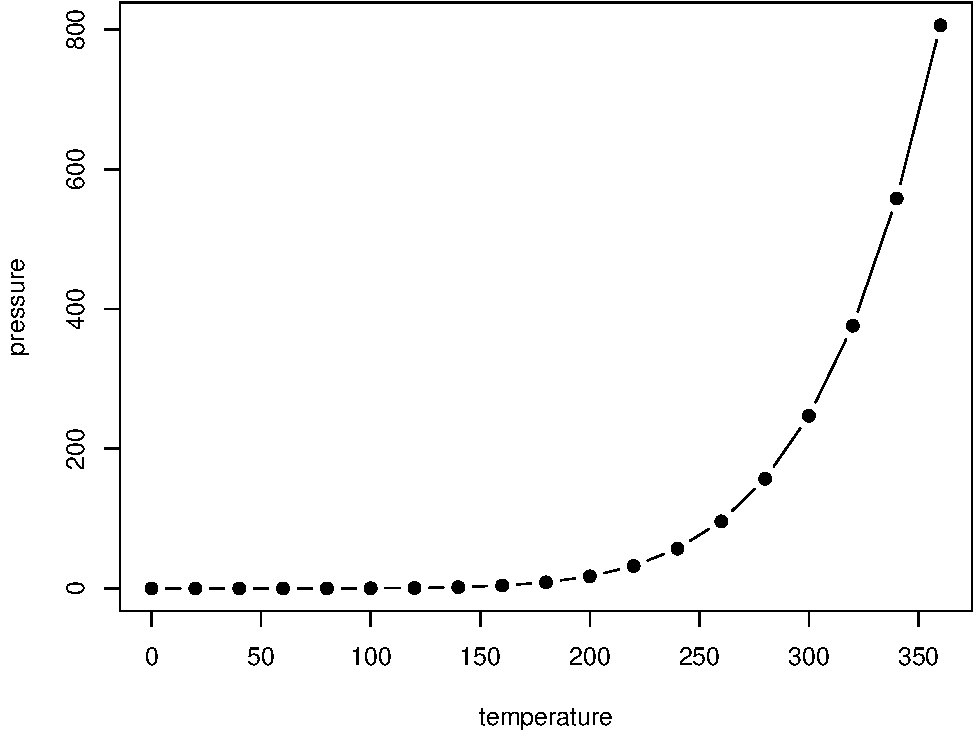
\includegraphics[width=0.8\linewidth]{03-cross-refs_files/figure-latex/nice-fig-1} 

}

\caption{Here is a nice figure!}\label{fig:nice-fig}
\end{figure}

Don't miss Table \ref{tab:nice-tab}.

\begin{Shaded}
\begin{Highlighting}[]
\NormalTok{knitr}\SpecialCharTok{::}\FunctionTok{kable}\NormalTok{(}
  \FunctionTok{head}\NormalTok{(pressure, }\DecValTok{10}\NormalTok{), }\AttributeTok{caption =} \StringTok{\textquotesingle{}Here is a nice table!\textquotesingle{}}\NormalTok{,}
  \AttributeTok{booktabs =} \ConstantTok{TRUE}
\NormalTok{)}
\end{Highlighting}
\end{Shaded}

\begin{table}

\caption{\label{tab:nice-tab}Here is a nice table!}
\centering
\begin{tabular}[t]{rr}
\toprule
temperature & pressure\\
\midrule
0 & 0.0002\\
20 & 0.0012\\
40 & 0.0060\\
60 & 0.0300\\
80 & 0.0900\\
\addlinespace
100 & 0.2700\\
120 & 0.7500\\
140 & 1.8500\\
160 & 4.2000\\
180 & 8.8000\\
\bottomrule
\end{tabular}
\end{table}

  \bibliography{book.bib,packages.bib}

\end{document}
